

\section{Experiment motivation}
The introduction lists several questions that this report should contribute to.
One of the questions concerns how collective decision making influences the emergence of self-assembly.
Swarm behaviour found in nature displays how simple agents collectively can make a decision.
The goal of this experiment is therefore to design a similar environment to promote this form of collective behaviour.
In this environment the robots have to form swarms for survival, and collectively decide if they should self-assemble or attempt an escape.

The experiment also allows investigation into the other questions this report contributes to.
By varying the parameters of the experiment it is possible to observe how different docking mechanisms and assembly protocols influence the self-assembly behaviour of the robots.
Section \ref{sec:results} further describes how this experiment can answer these questions.
\section{Experiment setup}
\label{sec:description}
For this experiment a micro-organism environment is imagined, where the organisms find themselves in some liquid pool. 
The micro-organisms are the agents in our system and are represented as swarm bots.
The main functions of the robots are, in addition to movement, foraging and self-assembly.

The robots find themselves in a pond.
In the pond there are nutrients which the robots can feed on to replenish their energy.
At the same time the pond also contains larger predator organisms which wants to feed on the robots.
It is imagined that the robots can assemble to form larger structures.
The robots can protect themselves from the predator organisms by forming a larger structure which the predator is unable to eat.
When the robots are assembled they may eat the larger predator to replenish energy as well.
The predators come in multiple sizes, and to gain an advantage the robots must form a large enough structure.
Maintaining the assembled structure cost energy, and the robots therefore have an incentive to disassemble once the structure is no longer required.

\section{Environment}
The imagined pond environment can be represented as a rectangular box(figure \ref{fig:environment}), containing the robots, nutrients and predators.
Initially the environment is populated with nutrients, robots, and predators placed at random positions in the environment.
When a nutrient is consumed, a new one is placed at a random position in the environment.
Additionally, to ensure fairness the predators cannot be placed within a threshold radius of a robot. 

\begin{figure}[H]
	
	\centering
	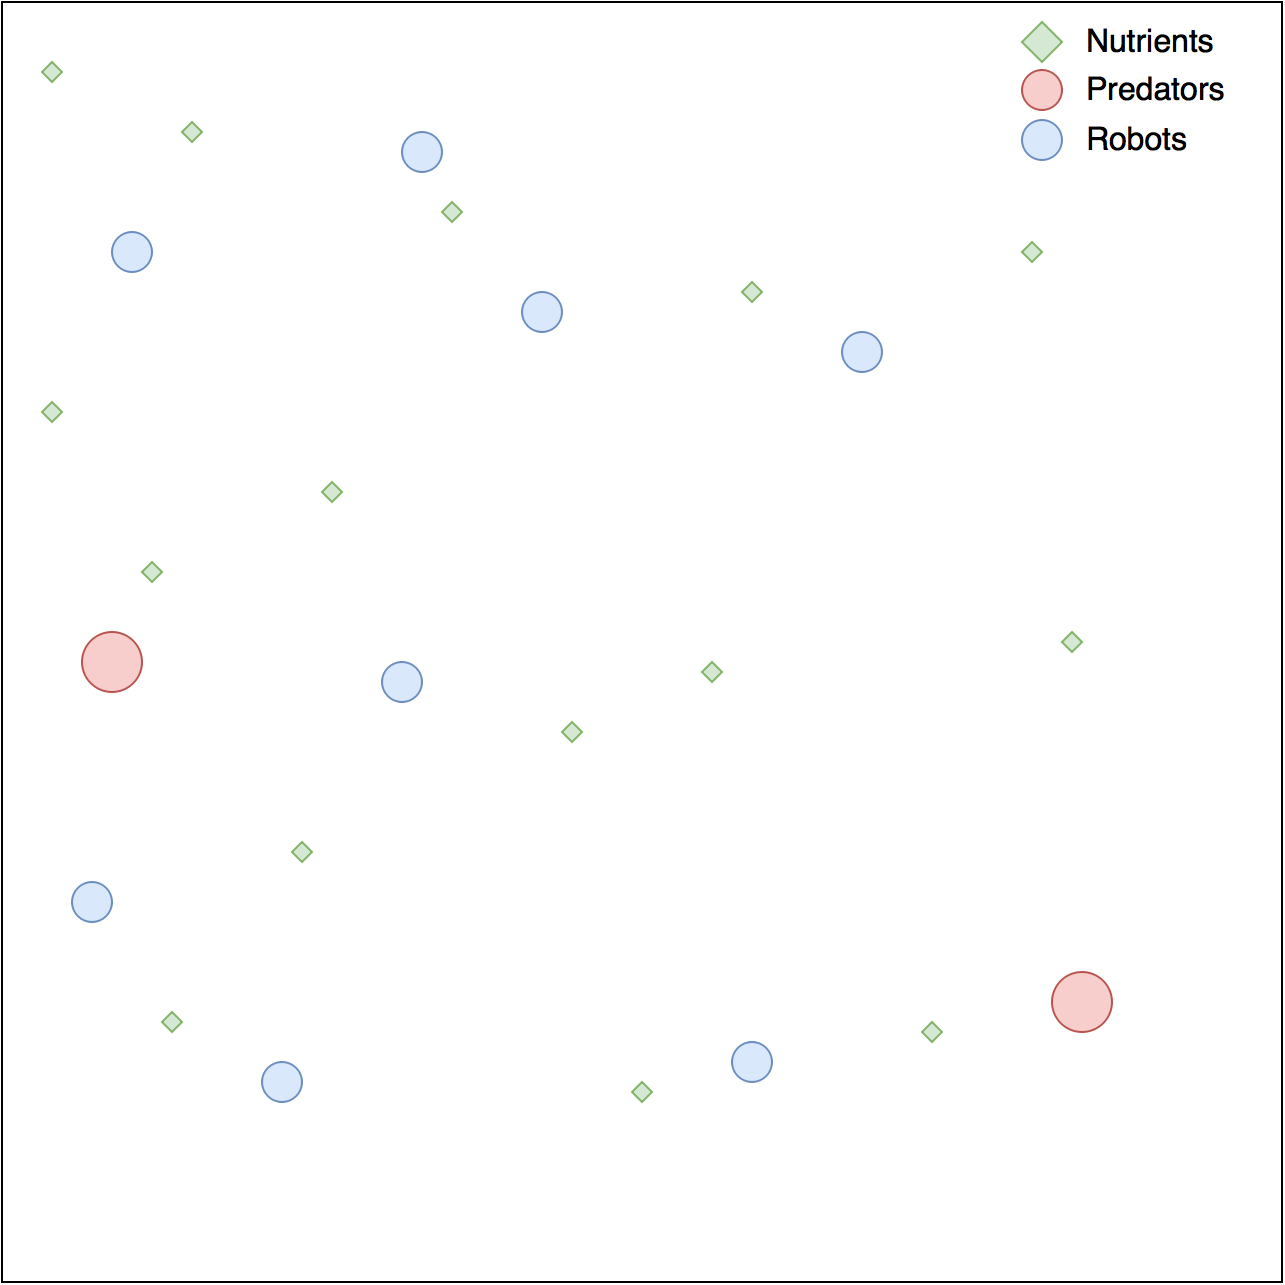
\includegraphics[width=0.65\textwidth]{chapters/res/Environment.png}
	\caption{Initial configuration of the environment.}
	\label{fig:environment}
\end{figure}

\section{Roborobo overview}
	\subsection{Agent observers}
	\subsection{Agent controllers}
	\subsection{World observers}

\clearpage

\section{Roborobo modifications}
	\subsection{Robot Groups}
	As mentioned in the description, roborobo does not support self-assembly out of the box.
	Self-assembly support therefore requires adding additional abstractions to roborobo.
	The high level abstraction that encapsulates the behavior for connected robots is called a \emph{Robot group}.
	All robots that are capable of self-assembly are robot groups.
	This means that single robots that are not connected are simply robot groups with one member.
	The responsibilities of the robot group is to take care of group movement, handling collisions, connecting and disconnecting. 
	\subsubsection{Movement}
	In the roborobo framework the robots movement is decided by the robot controller by requesting a certain angular and translational velocity.
	The movement of a group is decided by first converting the desired direction and velocity into a translation vector.
	\begin{equation}
		\centering
		\vec{v_{xy}} = v\cdot[\cos(\theta), sin(\theta)]
	\end{equation}
	The combined movement for the group is then decided by averaging the translation vectors from each member in the group.
	\begin{equation}
		\centering
		\vec{v_t} = \frac{1}{n}\sum_{i=0}^{n} \vec{v_{i}}
	\end{equation}
	Once the translation vector for the group is computed it can be applied to each member of the group by converting it back to the format of direction and velocity that roborobo uses.
	
	\subsubsection{Collisions}
	Roborobo already performs collision detection for robots, but in robot groups some additional logic is required.
	The collision behavior for robots is that if they collide with a solid object, they stop.
	This is a problem for groups of more than one robot because if one robot collides it may get left behind by the rest of the group.
	This is solved by backing up the position of each robot in a group before applying the computed translation.
	If a robot in the group collides with something, the robots in the group are reverted to their original position.
	\subsubsection{Connections}
	It is useful to treat the connections between robots in a group as a graph, where the robots are nodes and connections are edges.
	Connecting robots can then be treated as simply adding an edge between the two nodes representing the robots.
	Similar to connecting, disconnecting consists of removing the edge between the nodes representing the robots.
	In the case that a robot has multiple connections in the group extra care has to be taken, because removing one edge may split the graph into two smaller sub-graphs.
	If this occurs the two sub-graphs must now be treated as two new separate groups.
	It can be determined if a robot can simply be disconnected, or if we have to split the group by finding out if there is a cycle that leads back to the robot that is to be disconnected.
	The existence of a cycle is determined by first removing the edge representing the connection, and then performing a depth first search.
	
	 
	\subsection{Docking mechanism}
	As described in section \ref{sec:mechanisms}, there is a wide variety of docking mechanisms used in previous projects.
	The docking mechanism implemented is therefore highly configurable, to support a wide variety of different mechanisms.
	The configurable properties are as following, the number of ports, the placement of ports, and different genders for the ports. 
	
	\subsubsection{Connection validation}
		The robots can attempt a connection at any time, this requires a procedure to make sure the attempted connections are valid.
		Before a connection can be established there are three requirements that have to be met.
		First, the ports have to be spatially sound. 
		Here the distance between the ports have to be less than a threshold value.
		
		\begin{equation}
		|\vec{p_1} - \vec{p_2}| < \epsilon
		\end{equation}
		
		Next, the position of the ports has to be geometrically sound.
		Here the angle between the ports have to fit within a threshold range.
		
		\begin{equation}
		 180 - \epsilon < |\theta_1 - \theta_2| < 180 + \epsilon
		\end{equation}
		
		Finally the gender of the ports must be compatible, meaning one of them is female while the other is male, or at least one of the ports being universal.
		
	\subsection{Local communication}
	The robots are equipped with a communication module that allows local communication with their connected neighbors.
	The message format is very simple, the robots can broadcast "packets" of floating point numbers.
	The size of the packets is equal to the number of connection ports.
	At the receiving end, the packets sent by neighbors are aggregated into a single packet.
	The aggregation is performed as adding the components of each packet with the corresponding components in the other packets. Figure \ref{fig:local_communication} illustrates this process.
	
	\begin{figure}[H]
		\centering
		\includegraphics[width=0.65\textwidth]{chapters/res/Local_communication.png}
		\caption{Robot B aggregating the messages received from robot A, and C.}
		\label{fig:local_communication}
	\end{figure}
	
	In the robot controller, the messages from the communication module is fed into dedicated message input neurons, and the value of the message output neurons are broadcast to the neighbours.

		
\subsection{Predators}
A crucial part of the environment in the simulation are the predator robots.
These robots are not under the influence of the evolutionary algorithm and rather uses a much simpler pre-programmed controller.
The predator robots have two basic actions that can influence the system: the predators can either eat prey or explore the envelopment.

\begin{figure}[H]
		\centering
		\frame{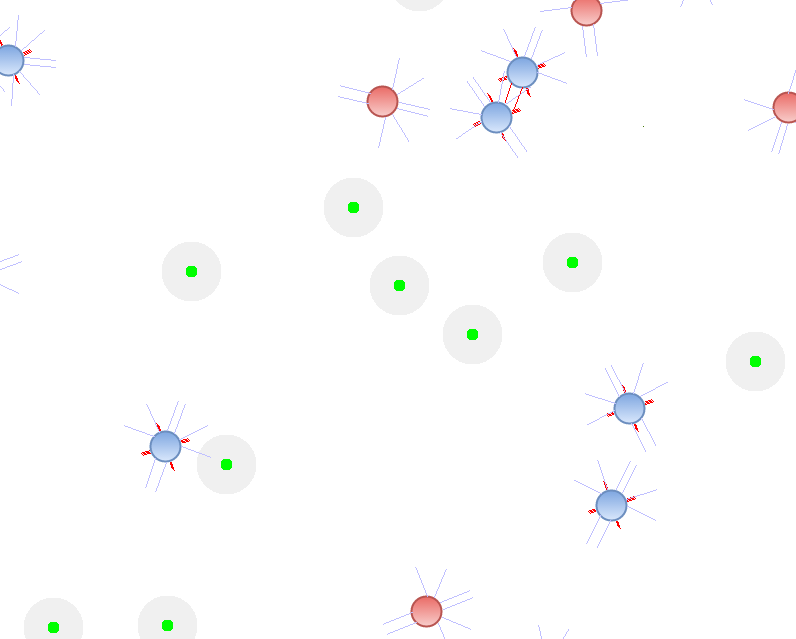
\includegraphics[width=0.65\textwidth]{chapters/res/predator_snippet.png}}
		\caption{A screenshot of a simulation. The predators are marked with red and the robots guided by the evolutionary algorithm are marked with blue}
		\label{fig:predator_screendump}
	\end{figure}

As seen in figure \ref{fig:predator_screendump}, the predators also uses six sensors which they use to decide if they are colliding with an object and what that object is.	
In terms of exploration, the predator controller uses a simple object avoidance tactic.
If the predator robots senses an object on any of its side sensors, it will change its rotational velocity to avoid this object.
In practice, this means that if the predator senses an object on the right, it will steer left, etc.
In the case where there is no collision, a slight random rotational velocity is added such that its movement is more dynamic.
This object avoidance behaviour is always employed as long as it does not sense a robot(prey).
In this case, it will have the opposite behaviour and turn towards the object, as it intends to consume the prey.

In addition to movement, the predators can also consume a robot. 
This happens when there is a collision between a normal robot and a predator robot.
If a robot is consumed, it is removed from the environment and amount of time it stayed alive is recorded for use in the fitness function of the evolutionary algorithm. 
For a predator to be able to eat a robot, the robot must not be part of a robot group of a size less then some configurable threshold.
The reason for this is to give the normal robots some advantage of self-assembling in hopes of potentially evolving this behaviour.  



\subsection{Energy drain}
\subsubsection{Passive}
\subsubsection{Active}
\clearpage
\section{CTRNN}
For this project, an artificial neural network that has gained a lot a popularity in regards to robotics known as Continuous-Time Recurrent Neural Network (CTRNN) was implemented. 
The CTRNN was researched and developed by Randall Beer and adds two new properties to the standard artificial neural network. 
The properties that are introduced in CTRNN is a time constant and a gain.

As most neural networks, the simple integration of the inputs from all neighbouring neurons are added giving us the first standard equation for neural networks:

\begin{equation}
	s_i = \sum_{j=1}^{n}o_{j}w_{i,j}+I_i
\end{equation}
\\
Here, $o_j$ represents the output(after activation) of neuron $j$, $w_{i,j}$ is the weight from neuron $j$ to neuron $i$ and $I_i$ is the sum of all the external inputs to node $i$.

\begin{equation}
\frac{dy_i}{dt} = \frac{1}{\tau_i}[-y_i + s_i + \theta_i]
\end{equation}
\\
In order to preserve the previous state of the ANN, the internal state is stored. 
$y_i$ denotes the internal state of neuron $i$.
To derive the next internal state, Beer computes $\frac{dy_i}{dt}$ as a combination of the next inputs and the current internal state of the node, where a time constant $\tau_i$ decides rate of drain. 
$\theta_i$ is a term added for neuron specific bias, but is only added here for mathematical soundness as it was simply added as a bias node during implementation and hence incorporated in $s_i$.
The time constant $\tau_i$ is what gives CTRNNs the ability to produce rich functionality and convincingly sophisticated cognition.
If $\tau_i$ has a low value then we will have a high degree of drain and hence having the next state being dominated by its new input.
However, if $\tau_i$ has a high value, then we have a higher degree of memory because it will be dominated by its previous state.

\begin{equation}
o_i = \frac{1}{1 + e^{-g_{i}y_{i}}}
\end{equation}
\\
To convert the internal state to an output $o_i$, Beer typically uses sigmoidal activation function.
This is typical in other neural networks as well, but Beer also employs a gain term $g_i$, to influence the activation of the neuron.
\\
\begin{figure}[H]
	\centering
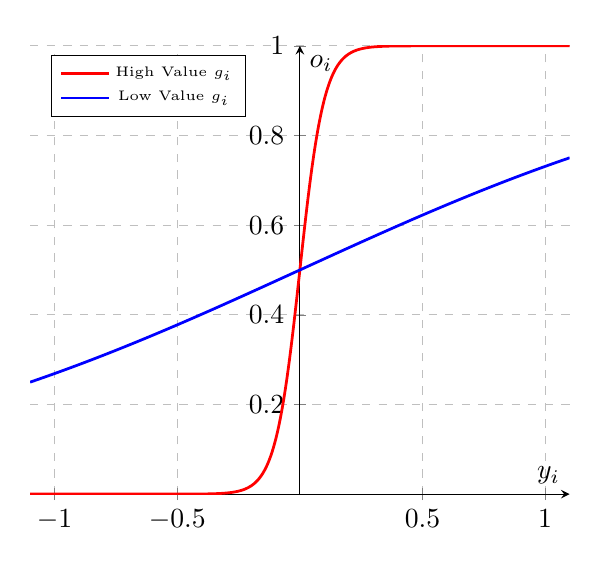
\begin{tikzpicture}
\begin{axis}[
	axis lines = center,
    xlabel = $y_i$,
    ylabel = {$o_i$},
    ymajorgrids=true,
    xmajorgrids=true,
    grid style=dashed,
    legend style={at={(0.22, 0.98)},anchor=north, font=\tiny}
]
%Below the red parabola is defined
\addplot [
    domain=-1.1:1.1, 
    samples=500, 
    color=red,
    line width=1pt,
]
{1/(1+e^(-20*x)};
\addlegendentry{High Value $g_i$}
%Here the blue parabloa is defined
\addplot [
    domain=-1.1:1.1, 
    samples=100, 
    color=blue,
	line width=1pt,
]
{1/(1+e^(-1*x)};
\addlegendentry{Low Value $g_i$}
 
\end{axis}
\end{tikzpicture}
	\caption{The difference in the activation function with respect to $y_i$ based on a low and high value of $g_i$}
	\label{CTRNN-gGraph}
\end{figure}

As seen in figure \ref{CTRNN-gGraph}, the value of the gain parameter can influence the activation function in such a way that it can be a smooth, almost linear, function or it can take on the behaviour of an activation function resembling a switch.
Having the ability to change the activation function on a neuron to neuron basis, is the second reason(the first being time constants) CTRNNs can give rise to complex and rich behaviour.



	\subsection{Drain}
	\subsection{Activation function}
	\subsection{Topologies}
		\subsubsection{Dense}
		\subsubsection{Sparse}
\clearpage
\section{Evolutionary algorithm}
	\subsection{Genotype}
	\subsection{Initialization}
	\subsection{Mutation operators}
		\subsubsection{Random}
		\subsubsection{Incremental}
	\subsection{Selection mechanism}
\clearpage
\section{Data gathering}
	\section{Loggers}
	\section{Analysis}
\clearpage
\subsection{Extras/Appendix?}
	\subsection{Parallelization}
	\subsection{Python graph tool}
	\subsection{System configuration}
\clearpage
	